\documentclass{article}
\usepackage[utf8]{inputenc}
\usepackage[icelandic]{babel}
\usepackage[T1]{fontenc}
\usepackage{graphicx}
\usepackage{mathtools}
\usepackage{amsmath}
\usepackage{amssymb}
\usepackage{minted}


\graphicspath{ {./} }
\title{snake - viðmótsforritun}
\author{ttb3@hi.is}
\date{\today}


\begin{document}
\maketitle


\section*{Skjáskot úr verkefni}
\begin{center}
    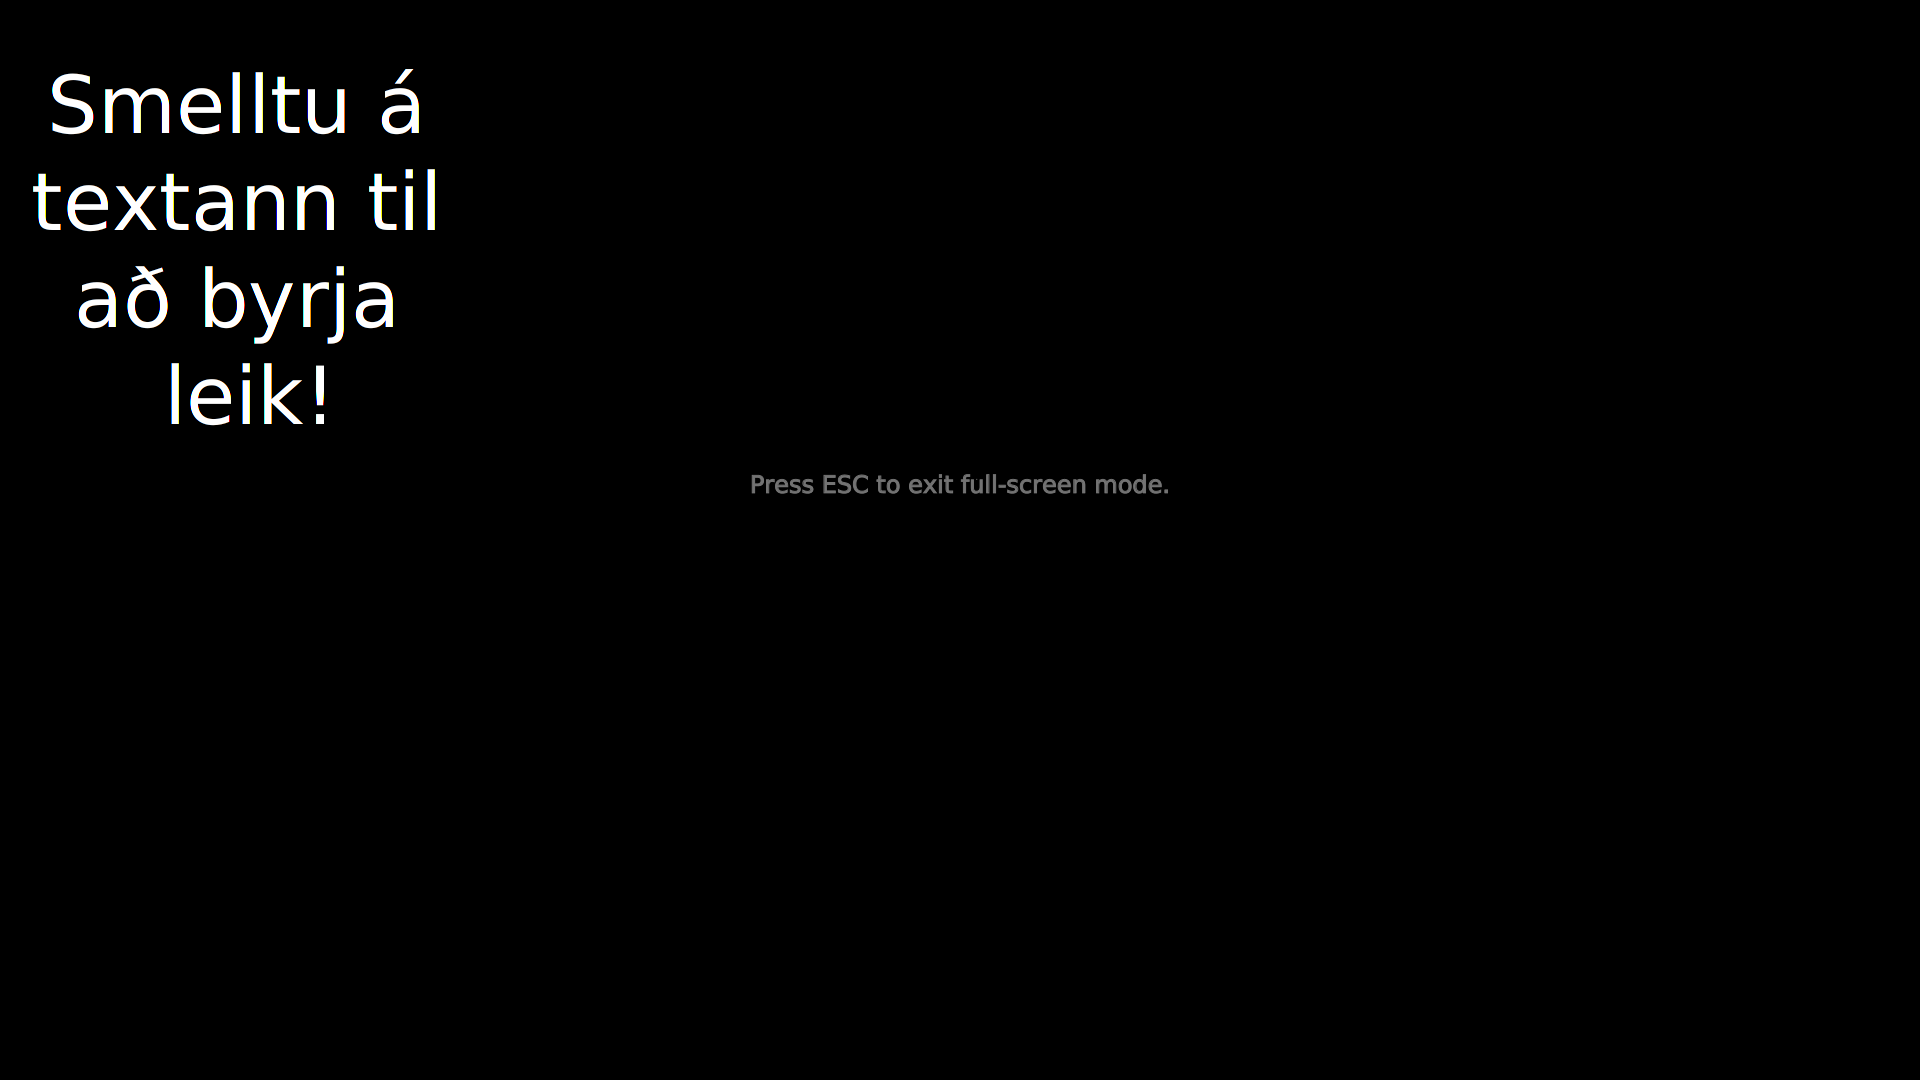
\includegraphics[scale=0.175]{sImg1.png}
\end{center}
þegar notandi byrjar keyrir forritið birtist þessi skjár, 
það er ekki mikið sem hægt er að gera hér, 
annað en að fylgja leiðbeiningum og smella á textann.
það sést líka ekki á screenshottinu, 
en það kemur upp texti frá stýrikerfinu sem segir notanda hvernig á að komast út úr leiknum,
ýta á escape takkann.

\begin{center}
    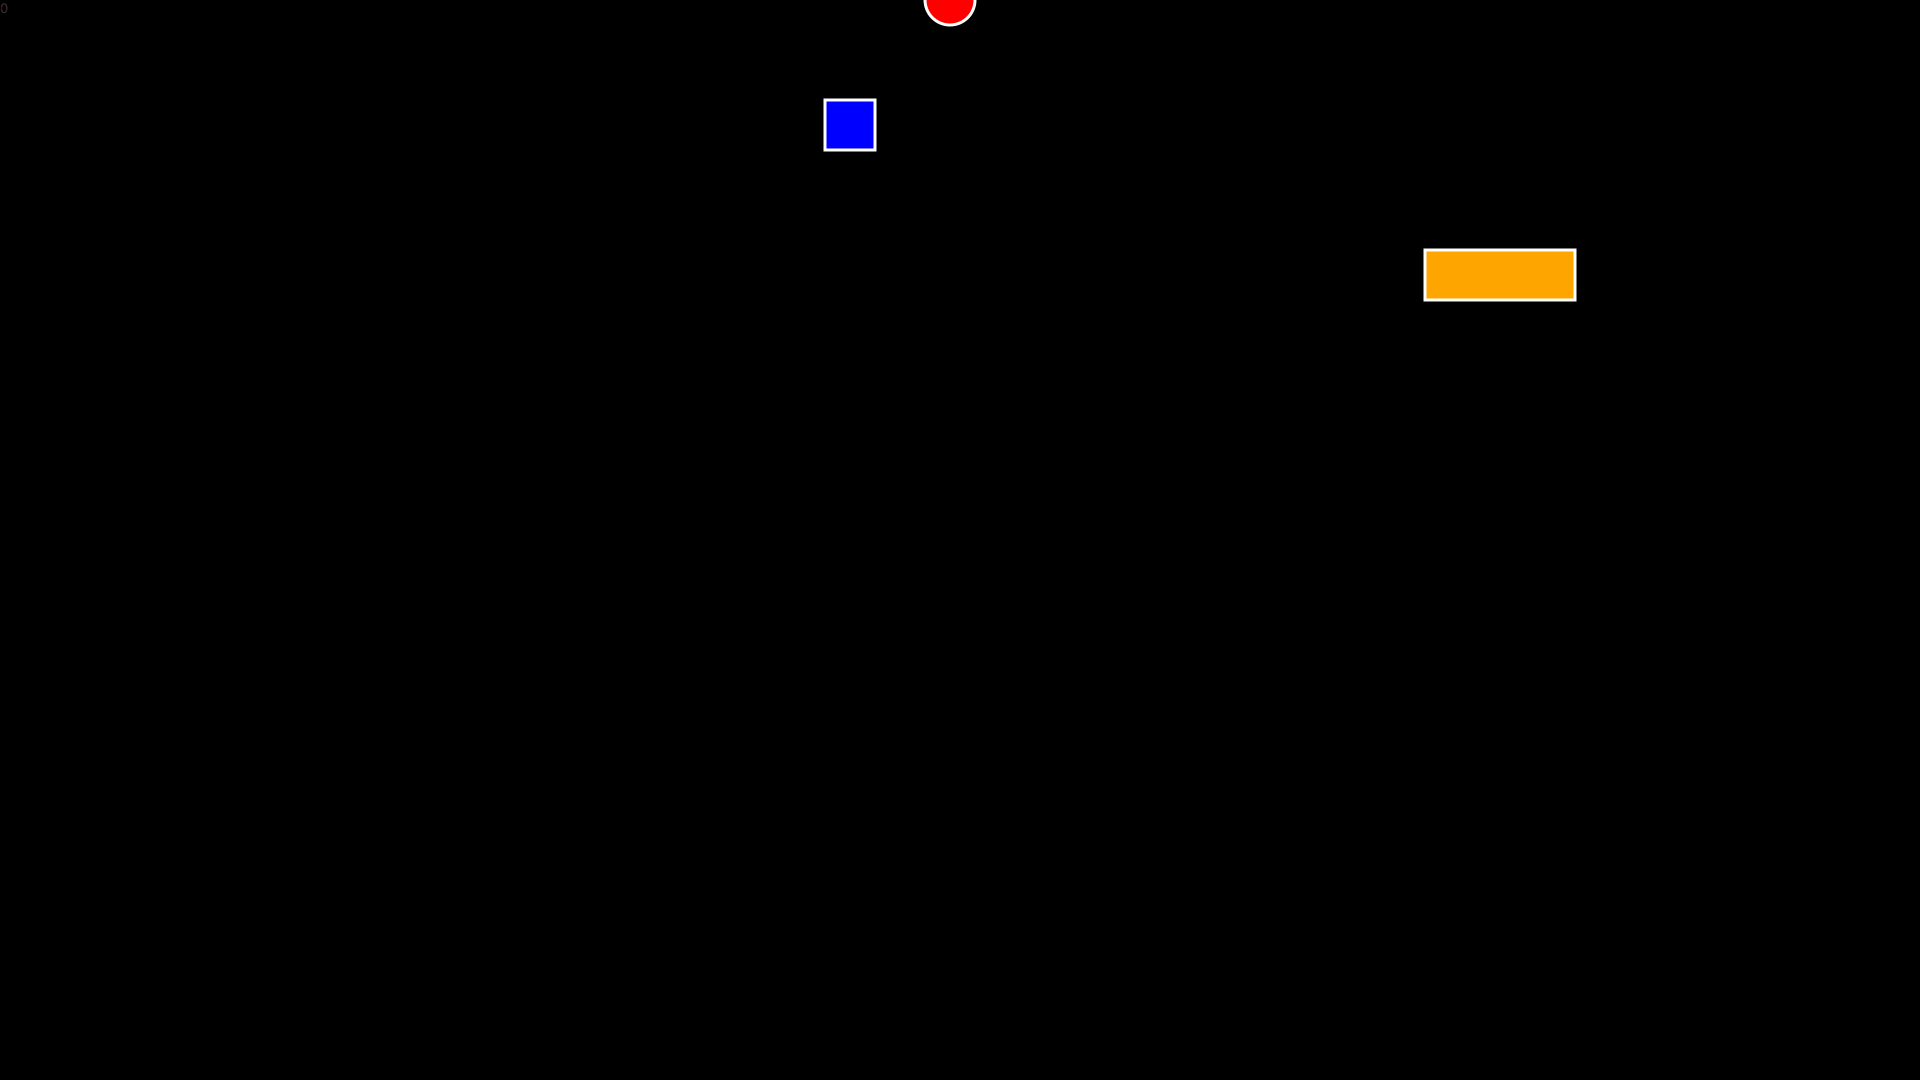
\includegraphics[scale=0.175]{sImg2.png}
\end{center}
leikurinn byrjar auðveldur, bara einn eitursnákur og enginn hali fyrir spilarann

\begin{center}
    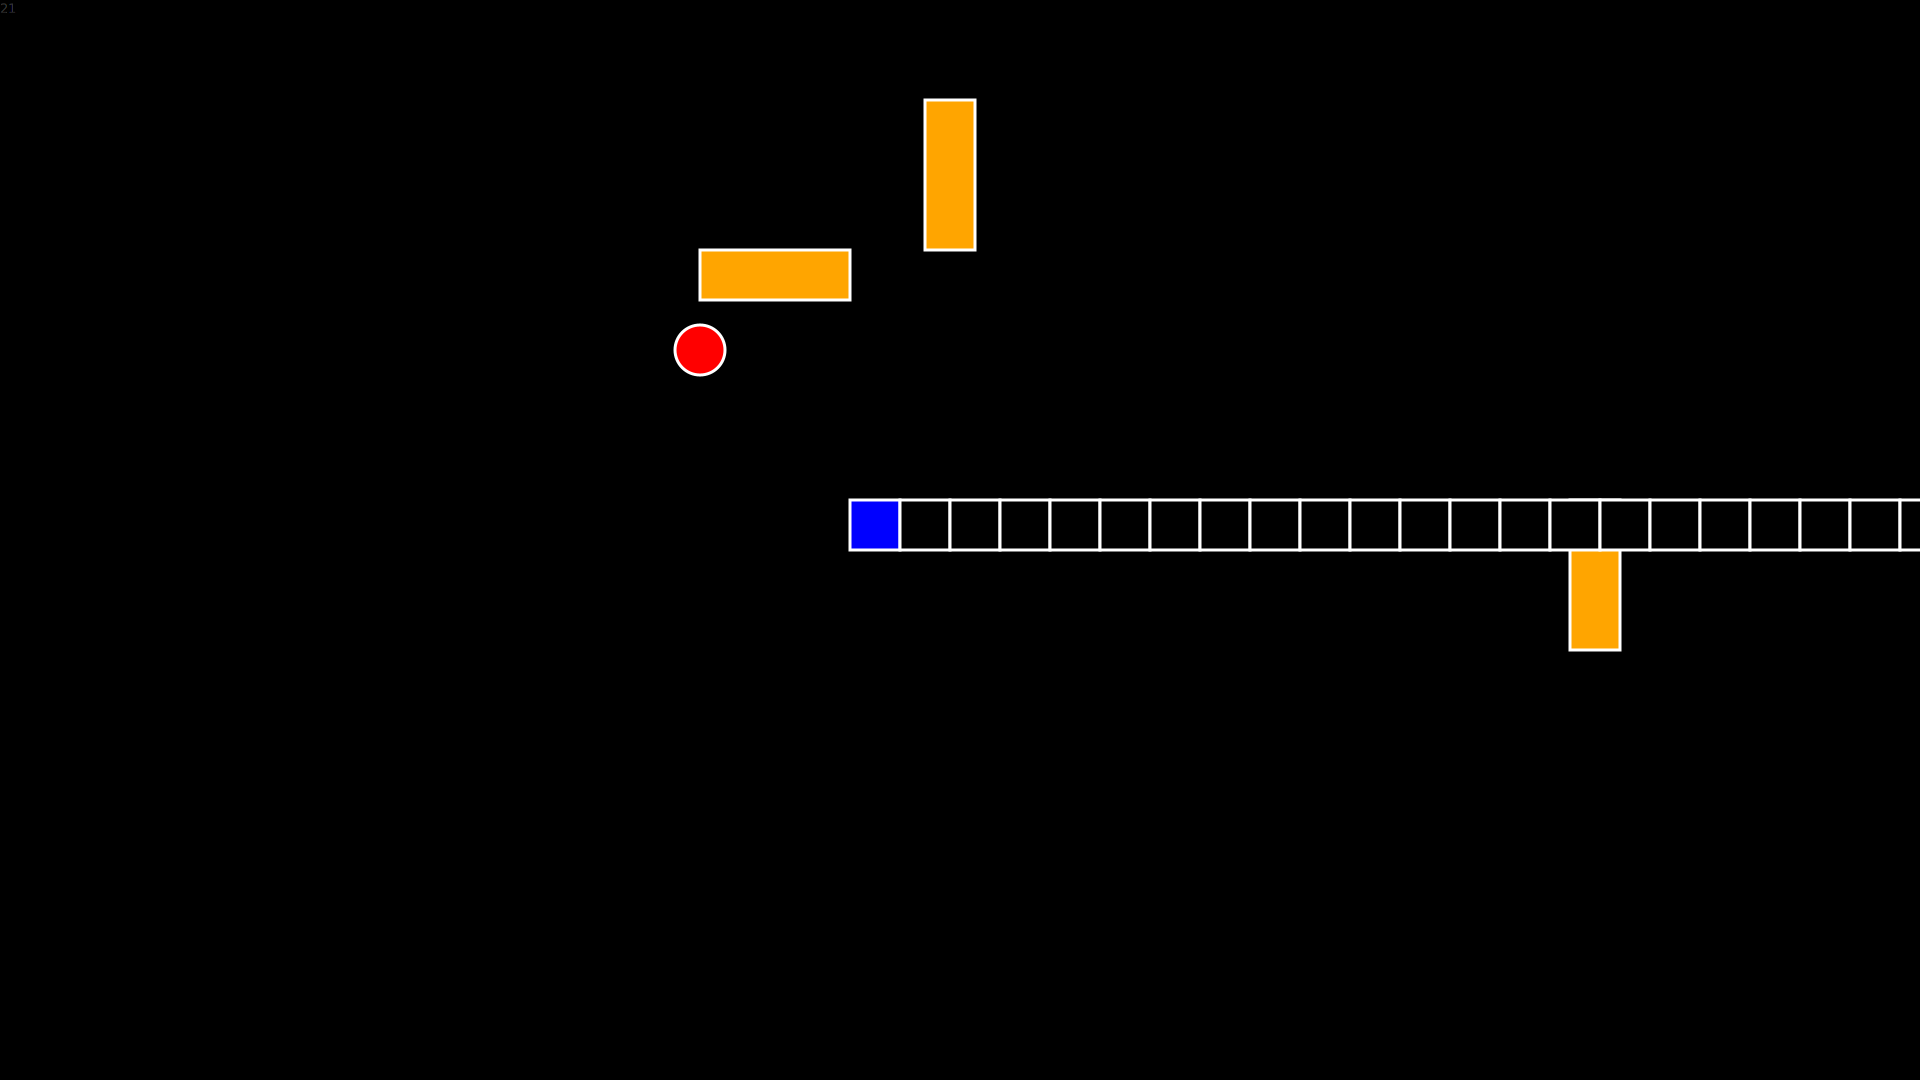
\includegraphics[scale=0.175]{sImg3.png}
\end{center}
hér er spilari kominn frekar langt, bæði komnir 3 eitursnákar og halinn orðinn býsna langur

\begin{center}
    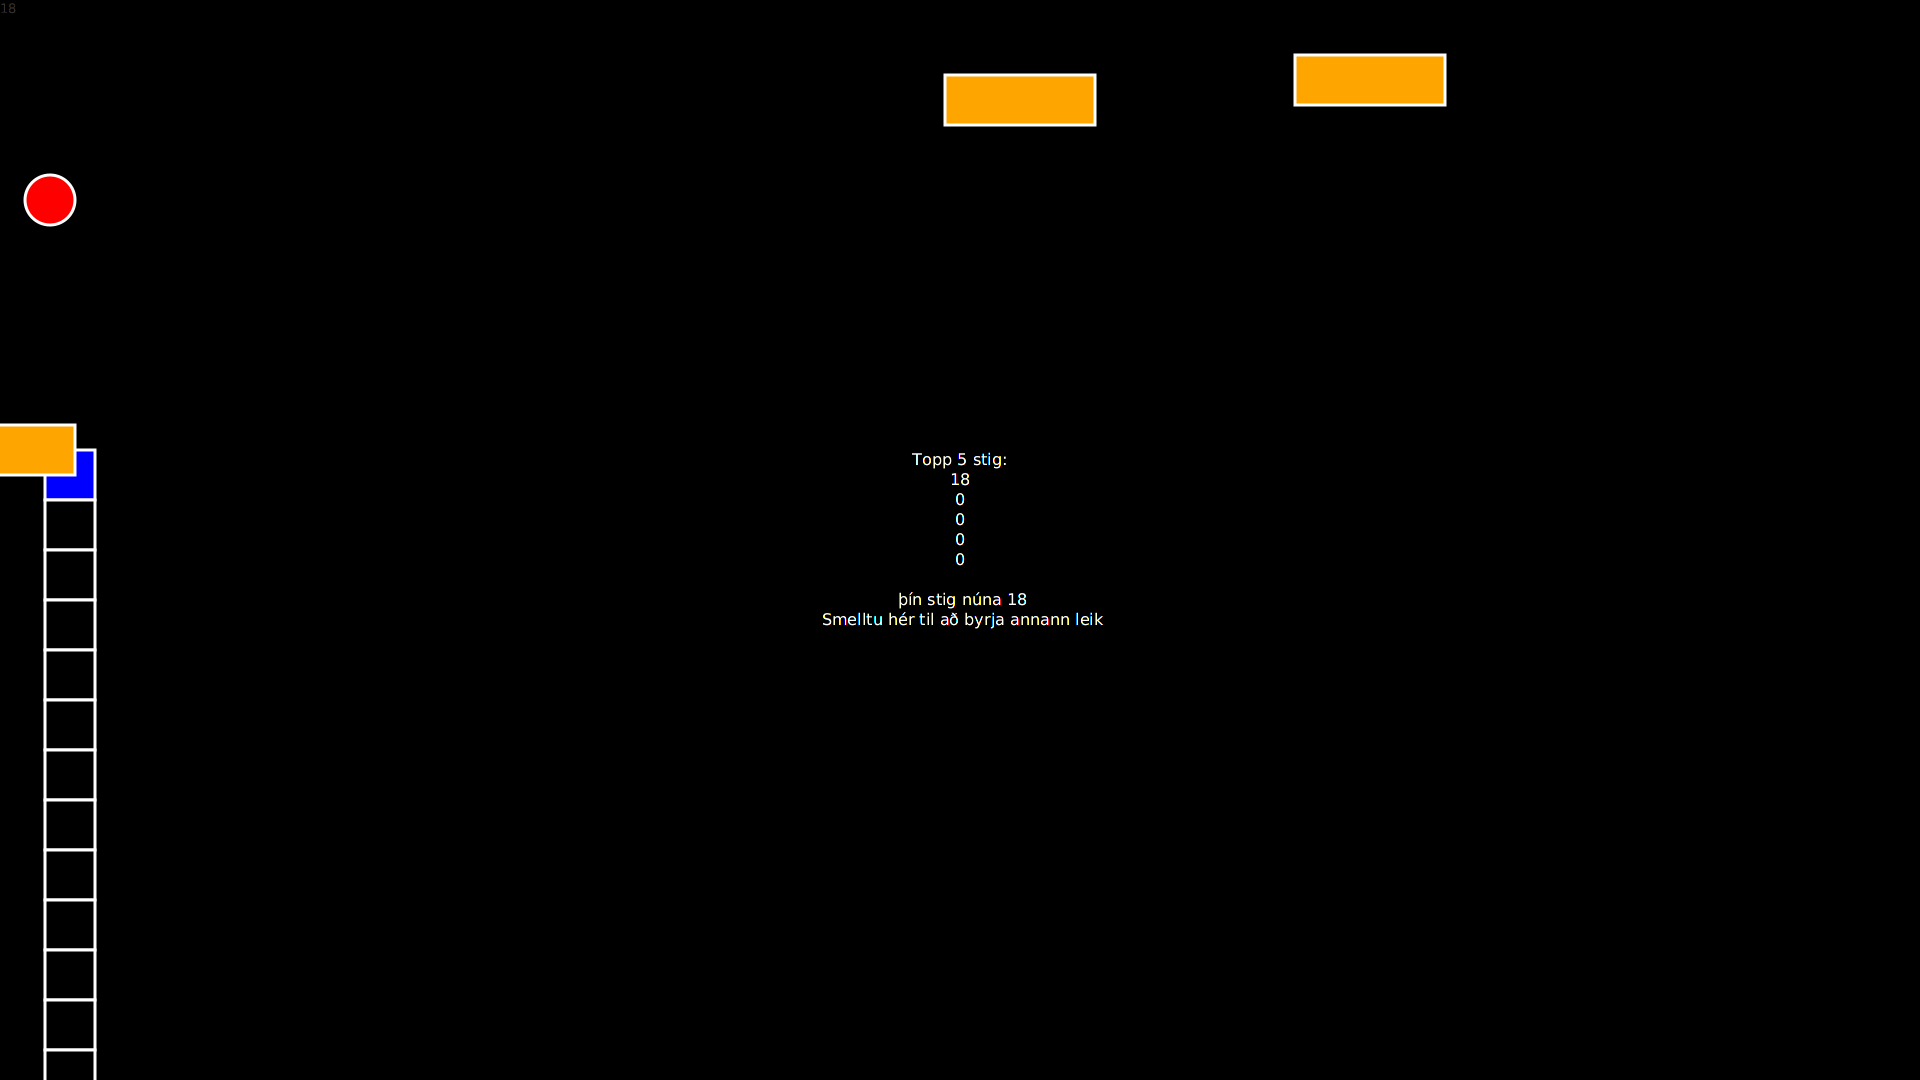
\includegraphics[scale=0.175]{sImg5.png}
\end{center}
en spilarinn flaug of nálægt sólinni og hrapaði á endanum, 
þegar spilari deyr birtist yfirlit yfir 5 bestu leiki á núverandi keyrslu forritsins

\section*{Teikningar gerðar í byrjun verkefnis}
\begin{center}
    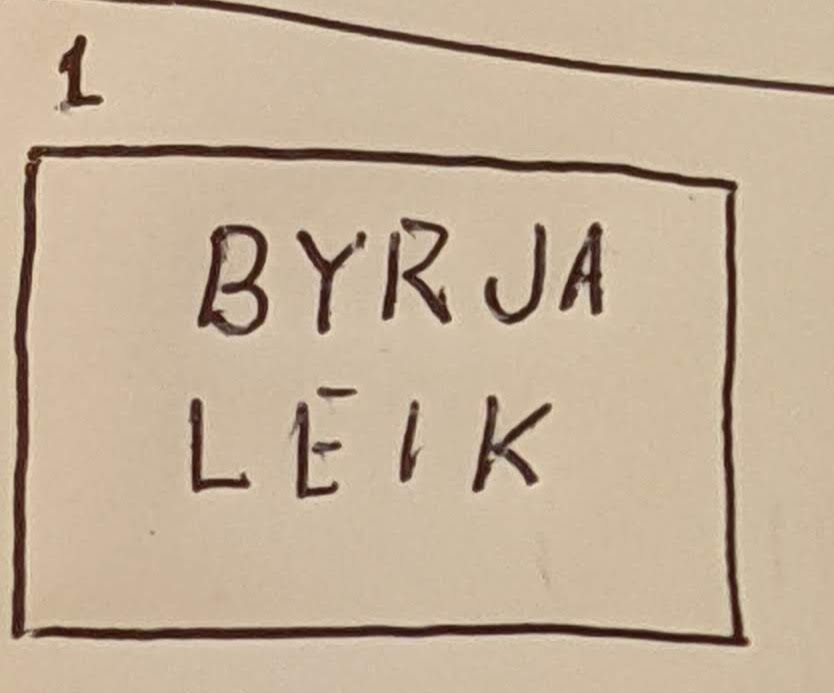
\includegraphics[scale=0.2]{t1.jpg}
    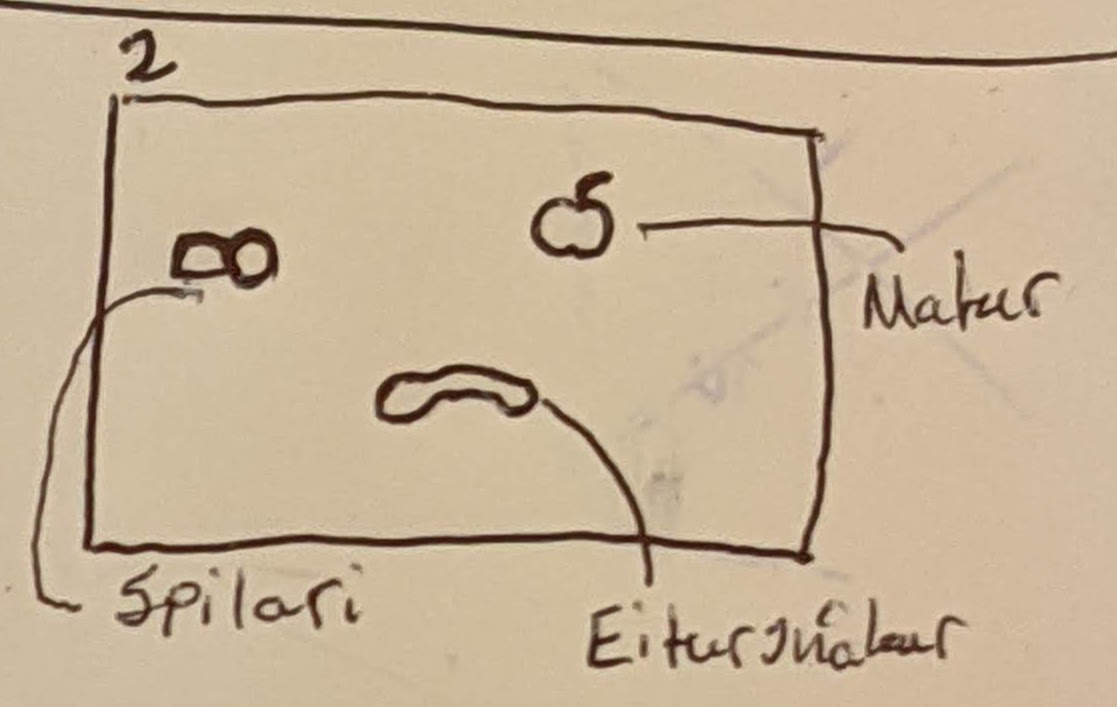
\includegraphics[scale=0.2]{t2.jpg}
    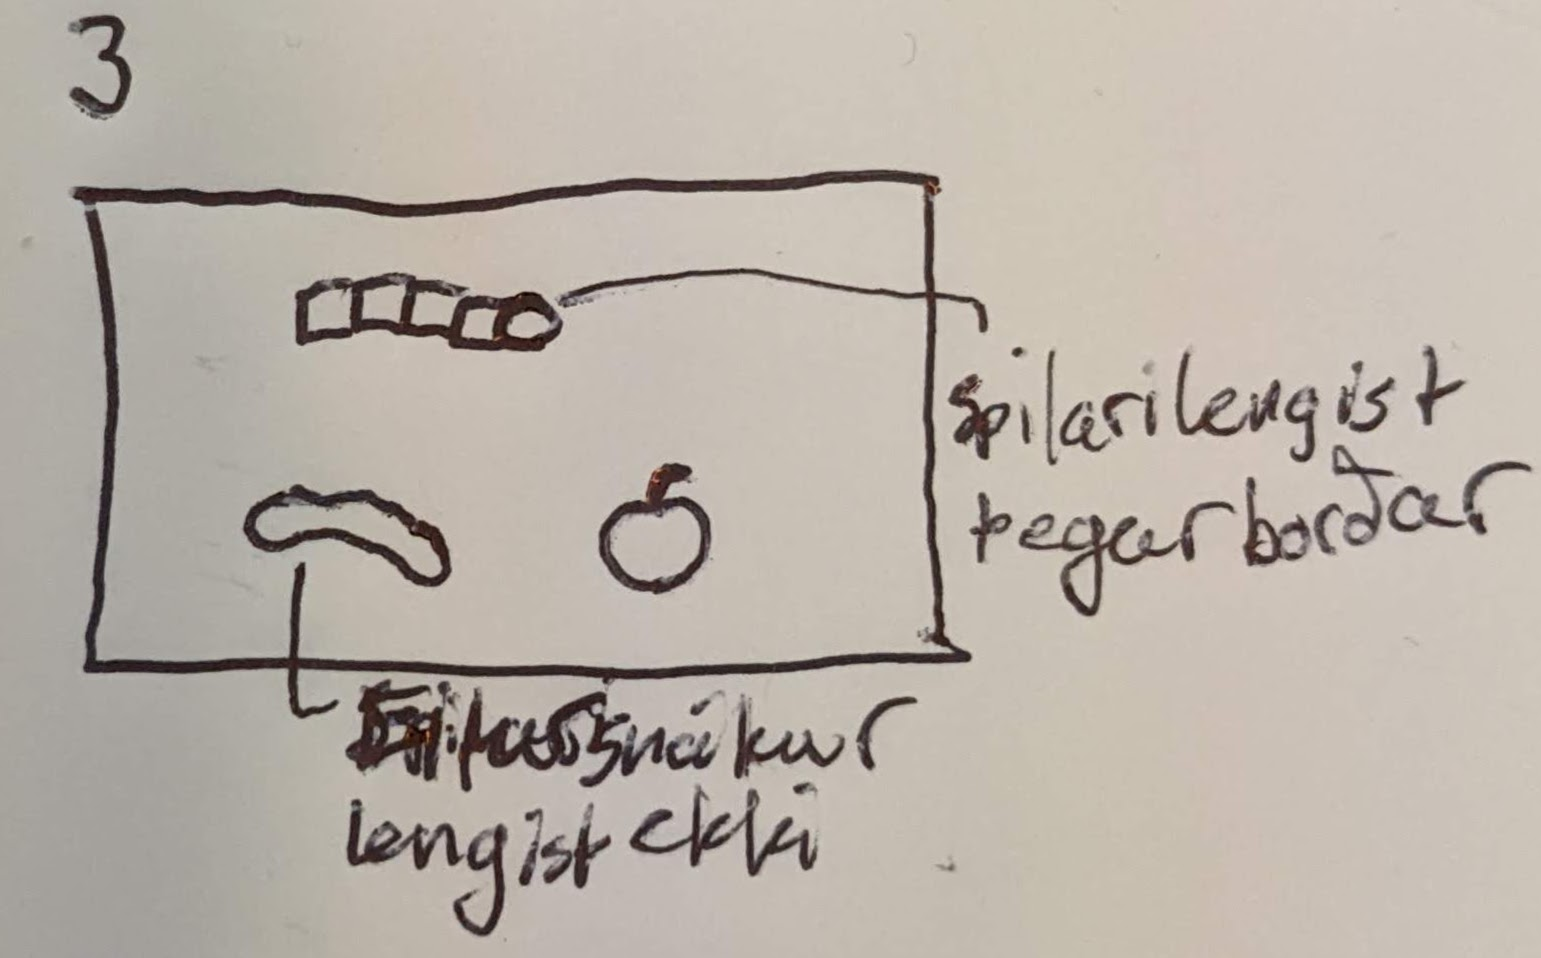
\includegraphics[scale=0.2]{t3.jpg}
    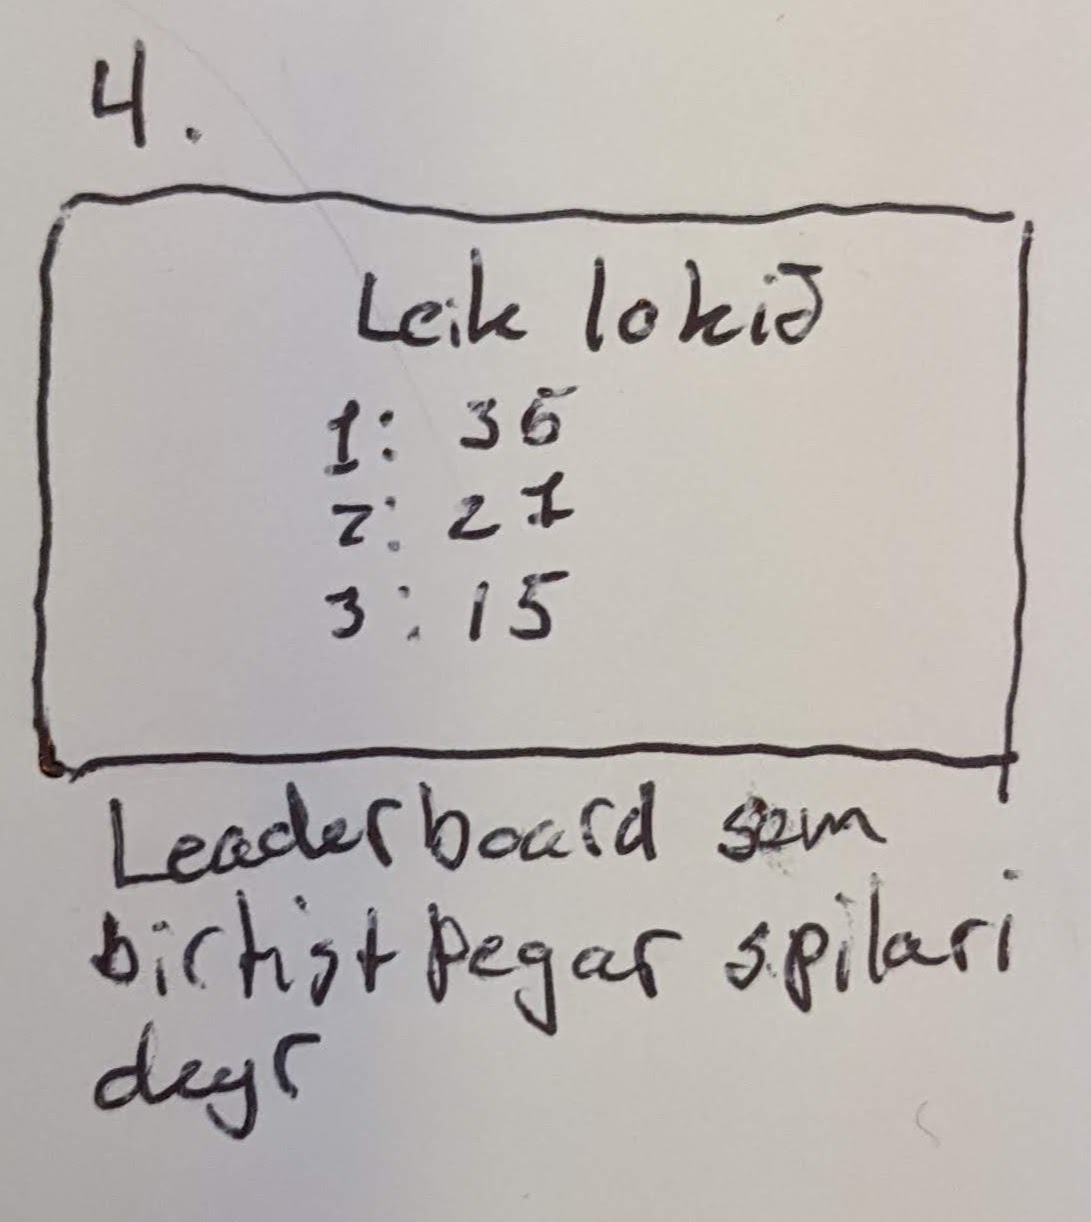
\includegraphics[scale=0.2]{t4.jpg}
\end{center}
\end{document}